\documentclass[12pt]{article}

\usepackage[margin=1in]{geometry}
\usepackage{amsmath,amsthm,amssymb}
\usepackage{fancyhdr}
\usepackage[small,compact]{titlesec}
\usepackage{float}

\lhead{Erich Menge}
\chead{\classnameandsection}
\rhead{\homeworktitle}

\pagestyle{fancy}

\newcommand{\sethomeworknumber}[1]{
  \newcommand{\homeworktitle}{Homework #1}
}

\newcommand{\N}{\mathbb{N}}
\newcommand{\Z}{\mathbb{Z}}
\newcommand{\homeworkheader}[1]{
  \title{\vspace{2in}\homeworktitle}
  \author{Erich Menge (X.500: menge053, Student ID: 4624713) \\
  #1}
  \maketitle
  \newpage
}

\newenvironment{problem}[1]{
  \ignorespaces
  \section*{Problem #1}
}{
  \ignorespacesafterend
}

\newenvironment{solution}{
  \ignorespaces
  \subsection*{Solution}
}{
  \ignorespacesafterend
}

\newcommand{\classnameandsection}{CSCI 4011 Formal Languages And Automata Theory Section 3}


\sethomeworknumber{7}

\begin{document}

\homeworkheader{\classnameandsection}

\begin{problem}{16.2-5}
  Describe an efficient algorithm that, given a set $\{ x_1,x_2,\ldots, x_n \}$ of points on the real line, determines
  the smallest set of unit-length closed intervals that contains all of the given points. Argue that your algorithm is
  correct.
  \begin{solution}
    We can implement a greedy alogorith to solve this problem much like the scheduling problem. Instead of selecting the
    activity that finishes first we can select the number that comes first on the number line.

    With our number line we have two optimal situations. One where there is an optimal solution in which the greedy
    choice is first, and one where we have an optimal solution where the greedy choice is not first. In the case the
    optimal solution doesn't have the greedy choice first, we can simply replace the first unit-length interval with the
    greedy choice.

    So first we do a quicksort on the numbers so that they are in order. We select the first number in sorted order and
    so then the interval $[x_1, x_1 + 1]$ is our greedy choice. The optimal solution then is the optimal solution to the
    subproblem with the greedy choice added onto it. The greedy choice then of our subproblem is the interval $[x_i, x_i
    + 1]$ of the next number that isn't overlapping.

    So our algorithm takes a sorted list, selects the first number and creates an interval $[x_1, x_1 + 1]$. It then
    iterates over the next $i$ numbers until it finds a number that isn't within the first interval. That is the second
    interval $[x_i, x_i + 1]$, it then continues to iterate this time comparing against the second interval. Since they
    are in sorted order we only need concern ourselves with the latest interval, the greedy choice. This is a fast
    algorithm, running in linear time.

    This algorithm is correct because the first interval starts at the first number and wastes no space to the left on
    the number line. Since each subproblem is handled this way, wasting no space on the left, the number of intervals is
    the smallest it can be (because there is no wasted space.) It is a linear time algorithm so it is very efficient.
  \end{solution}
\end{problem}

\begin{problem}{16.2-7}
  Suppose you are given two sets $A$ and $B$, each containing n positive integers. You can choose to reorder each set
however you like. After reordering, let $a_i$ be the $i$th element of set $A$, and let $b_i$ be the $i$th element of set
B. You then receive a payoff $\displaystyle\prod\limits_{i = 1}^n a_i^{b_i}$ . Give an algorithm that will maximize your
   payoff. Prove that your algorithm maximizes the payoff, and state its running time.
\end{problem}

\begin{problem}{16.3-2}
  Prove that a binary tree that is not full cannot correspond to an optimal prefix code.
  \begin{solution}
    \begin{proof}
      An optimal prefix code saves the most space and therefore corresponds to a tree of minimum depth. \\ Assume that a
      not-full binary tree corresponds to an optimal prefix code. \\ If we have a non-full sub-tree such as in the
      figure below, we can take one of nodes and move it up, shortening the path of that node without affecting the
      other nodes in the tree. Because the shortened path is more efficient, we conclude by contradiction that the non-
      full tree must not correspond to an optimal prefix code. \qedhere
      \begin{figure}[H]
        \centering
        \caption{Trees}
        \subfigure[Non-full Tree]{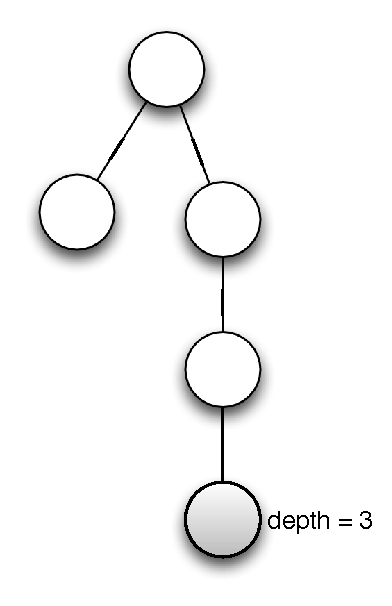
\includegraphics[scale=.75]{problem_16_3_2_a.eps}}
        \subfigure[Full Tree]{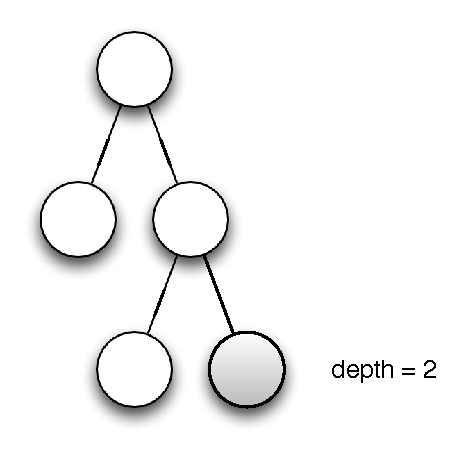
\includegraphics[scale=.75]{problem_16_3_2_b.eps}}
      \end{figure}
    \end{proof}
  \end{solution}
\end{problem}

\begin{problem}{16.3-3}
  What is an optimal Huffman code for the following set of frequencies, based on the first 8 Fibonacci numbers?
  \br
  a:1 b:1 c:2 d:3 e:5 f:8 g:13 h:21
  \br
  Can you generalize your answer to find the optimal code when the frequencies are the first n Fibonacci numbers?
\end{problem}


\end{document}
